\documentclass{beamer}

\setbeamercovered{transparent}

\usepackage{amssymb,amsmath}
\usepackage{natbib}
\bibliographystyle{apalike}
\usepackage[utf8]{inputenc}


\title{Interpolation Multidimensionnelle}
\author{Encadrant sénior : Laure Quivy\\Encadrant junior : Emile Contal}
\date{}

\setbeamertemplate{navigation symbols}{}
\makeatletter
\newenvironment{withoutheadline}{
  \setbeamertemplate{headline}[default]
  \setbeamertemplate{footline}[default]
}{}
\makeatother



%%%%%%%%%%%%%%%%%%%%%%%%%%%%%%%%%%%%%%%%%%%%%%%%%%%%%%%%%%%%%%%%%%%%%%%%%%%%%%%%
\begin{document}

\begin{withoutheadline}
\begin{frame}
\titlepage
\end{frame}
\end{withoutheadline}

%%%%%%%%%%%%%%%%%%%%%
\begin{frame}
  \begin{center}
    
\includegraphics[height=.15\textheight]{tdf.jpg}\\
    \vspace{\fill}
    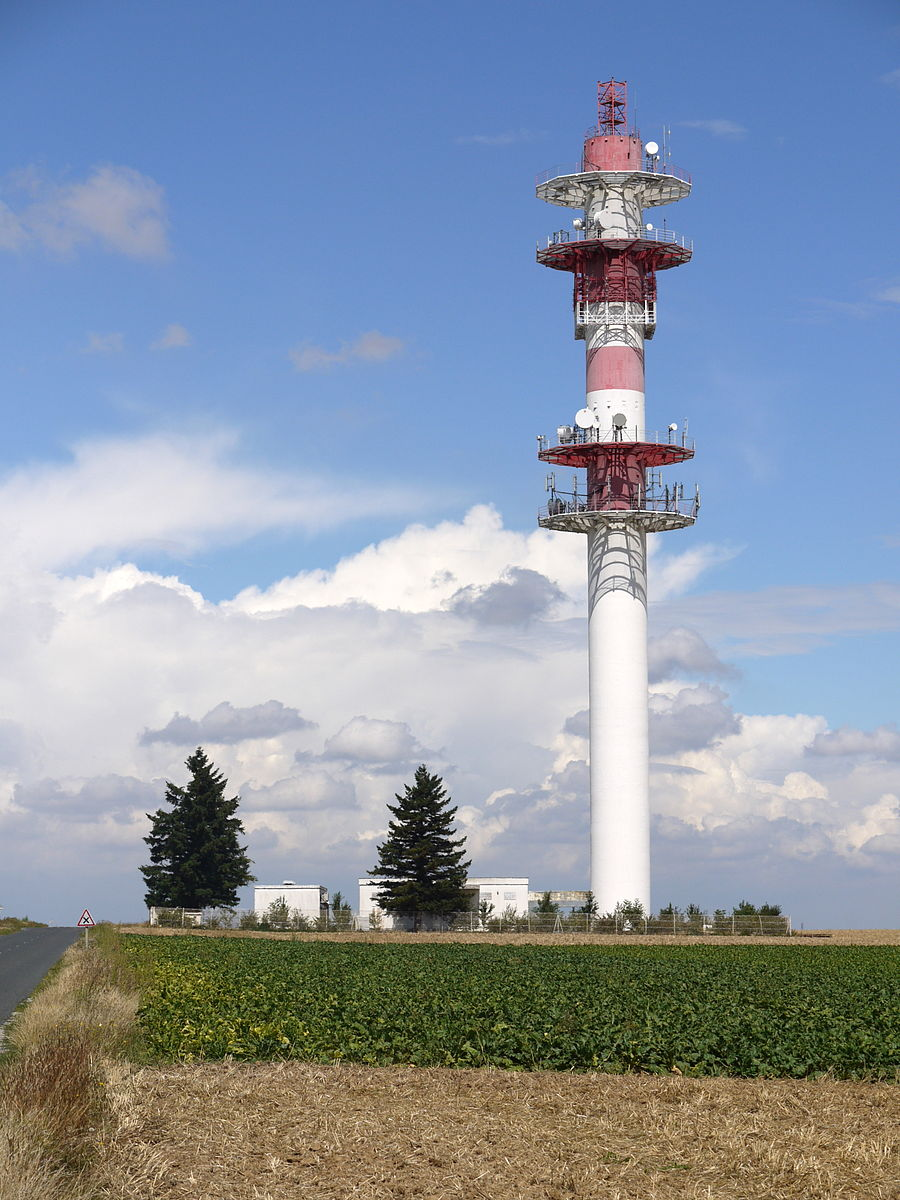
\includegraphics[height=.5\textheight]{relais.jpg}
    ~~~~
    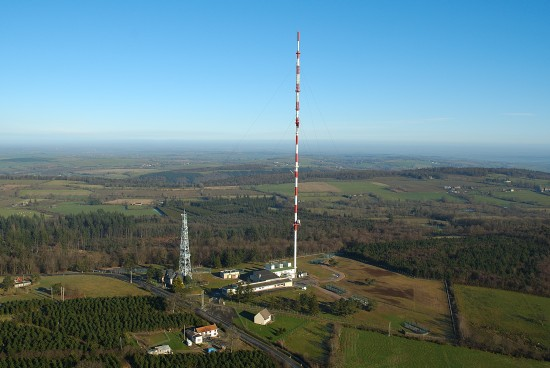
\includegraphics[height=.5\textheight]{pylone.jpg}
  \end{center}
\end{frame}

\begin{frame}
\frametitle{Enjeu}
\begin{block}{TDF (TéléDiffusion de France)}
  \begin{itemize}
  \item Vend l'utilisation de ses infrastructures (pylônes, antennes, \dots)
    aux opérateurs de diffusion de la TNT
  \item Le tarif de chaque site est soumis à un plancher 
    interdisant TDF de proposer des tarifs éliminant la concurrence
  \item Le calcul des tarifs planchers consomme beaucoup de temps
  \end{itemize}
\end{block}
\begin{block}{Approximation du tarif d'éviction}
  \begin{itemize}
  \item En fonction des caractéristiques du site (type d'antenne, puissance, \dots)
    on veut pouvoir calculer rapidement une estimation du tarif plancher
  \item 4 tarifs à calculer pour chaque site :
    un par an pendant 4 ans
  \end{itemize}
\end{block}
\end{frame}

\begin{frame}
\frametitle{Machine Learning}
\begin{block}{Maîtrise des méthodes de prédiction statistiques}
  \begin{itemize}
  \item Interpolation (ex: splines)
  \item Régression non-linéaire par noyaux
  \item Krigeage (régression par processus Gaussiens)
  \end{itemize}
\end{block}
\begin{block}{Comparaison et analyse des méthodes de prédiction}
  \begin{itemize}
  \item Évaluer la pertinence des modèles statistiques
  \item Comparer leur performances sur les données réelles
  \end{itemize}
\end{block}
\end{frame}

\begin{frame}
\frametitle{Enjeux avancés}
\begin{block}{Multi-objectif}
  Adapter les méthodes statistiques pour estimer 4 tarifs simultanément
\end{block}
\begin{block}{Interactions avec TDF}
  \begin{itemize}
  \item Rencontres chez TDF
  \item L'algorithme final sera développé en production
  \end{itemize}
\end{block}
\end{frame}

\begin{frame}
\frametitle{Enjeux avancés (suite)}
\begin{block}{Apprentissage actif}
  Construire (étendre) intelligemment la base des données réelles
  pour accélérer et améliorer l'apprentissage
\end{block}
\end{frame}



\end{document}
